\documentclass{report}
\usepackage[utf8]{inputenc}

\title{
    Sistema antifurto per veicoli - FindME \\
    \large Applicazioni e Servizi Web
}

\author{Davide Crisante - 0001044805 \{davide.crisante3@studio.unibo.it\}}
\date{\today}
\renewcommand\thesection{\arabic{section}}

\usepackage{natbib}
\usepackage{graphicx}

\graphicspath{ {./images/} }
\usepackage{caption}
\usepackage{subcaption}
\usepackage{dirtree}
\usepackage{float}
\usepackage{hyperref}


\begin{document}

\maketitle


\section{Introduzione}
FindME è un servizio web che consente di monitorare la posizione del proprio veicolo grazie a un dispositivo fisico da installare all'interno della vettura.\\
L'hardware del dispositivo comprende:
\begin{itemize}
    \item scheda SIM che permette la comunicazione via internet con il server;
    \item ricevitore GPS per determinarne la posizione;
    \item antenna per comunicare con un beacon che l'utente deve sempre portare con se quando utilizza il veicolo equipaggiato con il dispositivo FindME;
    \item batteria.
\end{itemize}

Il dispositivo manda il proprio stato (batteria residua, posizione, qualità del segnale GPS e internet) ai server FindME con cadenza regolare. Se il veicolo è in movimento e non viene individuato il beacon nelle vicinanze il dispositivo segnala il possibile furto al server e comunica il suo stato con una frequenza maggiore.\\
L'utente può monitorare lo stato del dispositivo dall'applicazione web e viene notificato in caso di presunto furto.
\newpage

\section{Requisiti}
In accordo con le moderne tecniche di \textit{Human-Computer Interaction} l'utente è stato considerato l'elemento fondamentale sul quale si è basata la progettazione dell'applicazione. Sono state quindi create delle \textbf{Personas} e degli \textbf{Scenarios} al fine di rappresentare un possibile gruppo di utenti di riferimento.
\begin{itemize}
    \item \textbf{Marco}\\studente universitario, 22 anni. Al momento lavora come fattorino usando la sua automobile. Quando va al mare è costretto a parcheggiare la sua auto molto lontano dalla spiaggia a causa della difficoltà nel trovare parcheggi liberi vicini nei weekend. Ciò mette non poche preoccupazioni a Marco, che dipende economicamente dallo stato della sua vettura senza la quale non potrebbe lavorare. Da qui la necessità di poter monitorare lo stato della propria vettura e di essere allertato in tempi brevi in caso di furto.

    \item \textbf{Giuseppe}\\pensionato, 65 anni. Dopo una lunga vita lavorativa da meccanico, Giuseppe continua a nutrire la propria passione per i motori restaurando veicoli d'epoca. Dopo anni di fatiche è riuscito a mettere a nuovo la sua prima auto che adora guidare e sfoggiare quando si sposta. Essendo un'auto molto rara Giuseppe sa che potrebbe essere rubata da qualche mal intenzionato e per questo non si allontana mai troppo da essa. Per questo motivo vorrebbe un sistema in grado di calmare le sue preoccupazioni mentre si diverte con i suoi ex-colleghi al bar.

    \item \textbf{Lisa}\\parrucchiera, 32 anni, non ama le nuove tecnologie. Da anni lavora in un salone all'interno di un centro commerciale. Un giorno uscendo dal lavoro si accorge che la sua auto non era più dove l'aveva lasciata, la ricerca tramite le forze dell'ordine non è stata fruttuosa e ora deve acquistare un'auto nuova. Questa volta Lisa vorrebbe tutelarsi tramite un sistema capace di riferirle dove si trovi la sua auto cosicché in caso di necessità possa fornire indizi utili alle forze dell'ordine per aiutarla a ritrovare la sua auto. Non vuole però che la sua posizione venga tracciata e salvata perché ciò la metterebbe a disagio.
\end{itemize}

Dallo studio delle personas e dei relativi casi d'uso è stato possibile individuare i seguenti requisiti.


\subsection{Funzionali}
\begin{itemize}
    \item registrarsi;
    \item effettuare login;
    \item visualizzare la posizione del dispositivo;
    \item visualizzare lo stato del dispositivo per rendersi conto sia della qualità del tracciamento che della necessità o meno di cambiare batteria;
    \item ricevere una notifica in caso di presunto furto;
    \item non immagazzinare dati sulla posizione non necessari.
\end{itemize}

Per mantenere il dispositivo operativo senza manutenzione il più a lungo possibile gli aggiornamenti possono non essere in tempo reale, ciò ci consente di utilizzare meno dati e meno energia.
\subsection{Non funzionali}
Le personas evidenziano il fatto che la principale fruizione del servizio verrebbe svolta per mezzo di un dispositivo mobile. Per questo la progettazione è stata svolta secondo l'approccio \textbf{Mobile First}, ideando quindi l'interfaccia per essere adeguata alla fruizione da dispositivi più limitanti (dispositivi mobili) in primo luogo e in secondo luogo per altri dispositivi (grazie all implementazione di un \textbf{design responsivo}). \\
Questo ha fatto sì che il design e i mockup siano stati incentrati sulla realizzazione di pagine adatte a dispositivi mobili da adattare successivamente a pagine più grandi come quelle di tablet o desktop.\\
Inoltre dati i nostri utenti di riferimento vogliamo un interfaccia semplice da utilizzare, intuitiva e reattiva.
\section{Design}
Il modello di design adottato è stato l' \textbf{User Centered Design} basato sulle \textbf{Personas} introdotte in precedenza. Il progetto è stato condotto seguendo una metodologia prevalentemente \textbf{Simil-Agile} caratterizzata da organizzazione ed esecuzione di \textit{Sprint} per ogni funzionalità da implementare.\\

\subsection{Design delle interfacce}
Il design delle interfacce è stato svolto cercando di sfruttare i principi \textbf{KISS} e \textbf{"Less is More"} al fine di realizzare un interfaccia semplice da fruire per gli utenti.\\
Di seguito sono riportati dei mockup realizzati per le sezioni ritenute più importanti dell interfaccia utente:

\begin{figure}[H]
   \begin{subfigure}{.5\textwidth}
  \centering
  \frame{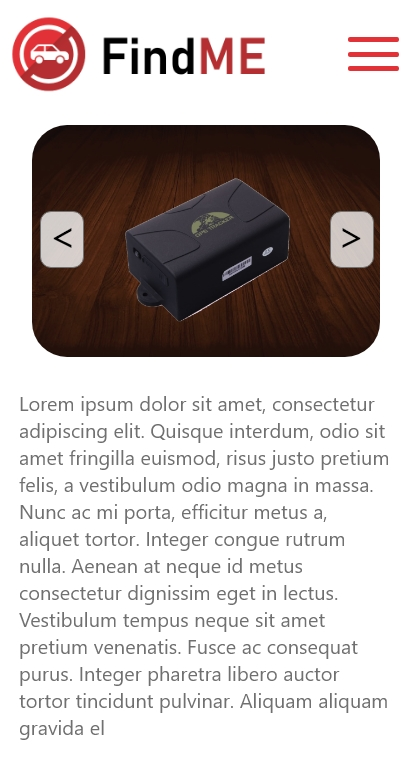
\includegraphics[width=0.9\linewidth]{img/home.jpg}}
  \caption{Public home}
  \label{fig:sub1}
\end{subfigure}%
\begin{subfigure}{.5\textwidth}
  \centering
  \frame{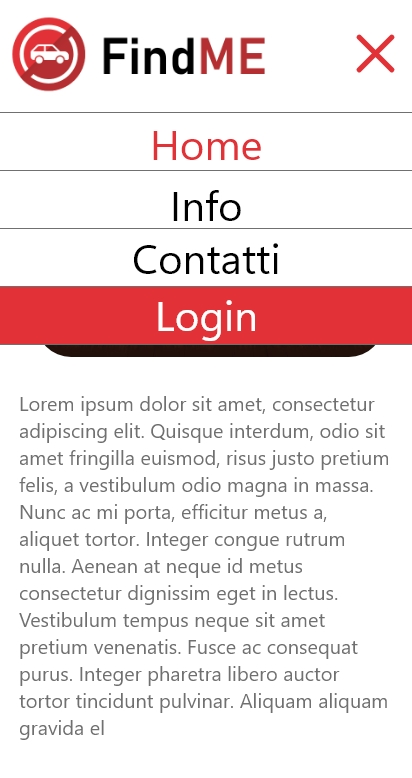
\includegraphics[width=0.9\linewidth]{img/home-menu.jpg}}
  \caption{Public home with menu opened}
  \label{fig:sub2}
\end{subfigure}
\caption{Public site home view}
\label{fig:test}
\end{figure}

\begin{figure}[H]
   \begin{subfigure}{.5\textwidth}
  \centering
  \frame{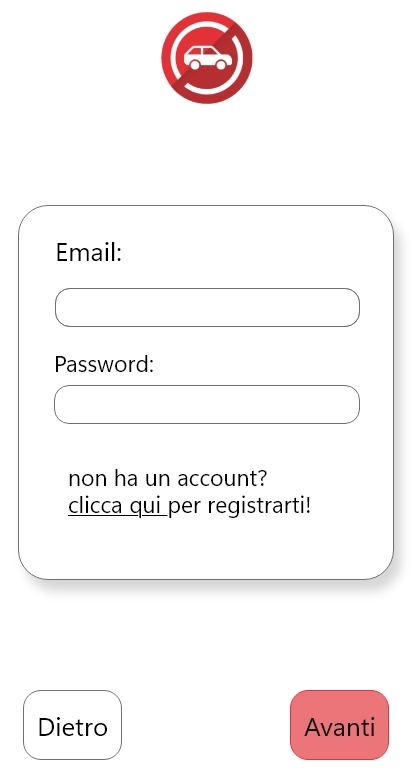
\includegraphics[width=0.9\linewidth]{img/login.jpg}}
  \caption{Login page}
  \label{fig:sub1}
\end{subfigure}%
\begin{subfigure}{.5\textwidth}
  \centering
  \frame{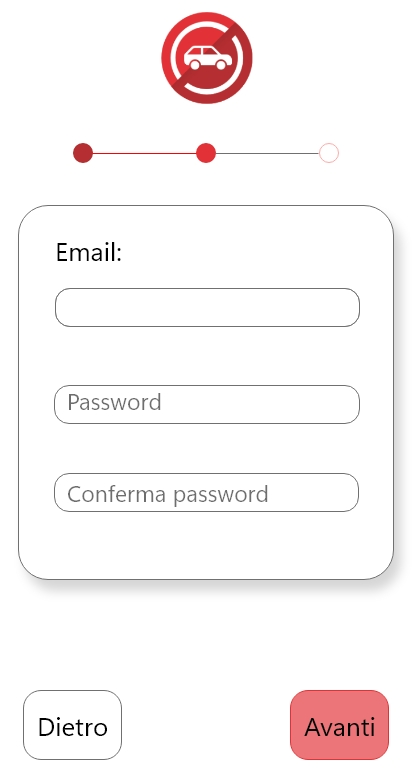
\includegraphics[width=0.9\linewidth]{img/signin.jpg}}
  \caption{Signin page}
  \label{fig:sub2}
\end{subfigure}
\caption{Login and signin view}
\label{fig:test}
\end{figure}

\begin{figure}[H]
   \begin{subfigure}{.5\textwidth}
  \centering
  \frame{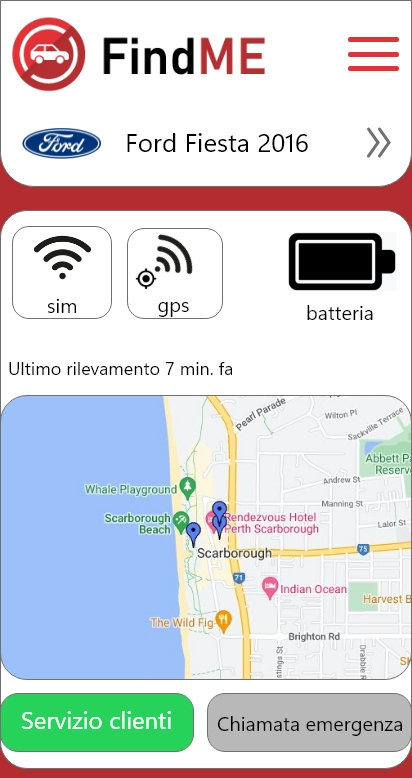
\includegraphics[width=0.9\linewidth]{img/dashboard.jpg}}
  \caption{Dashboard home}
  \label{fig:sub1}
\end{subfigure}%
\begin{subfigure}{.5\textwidth}
  \centering
  \frame{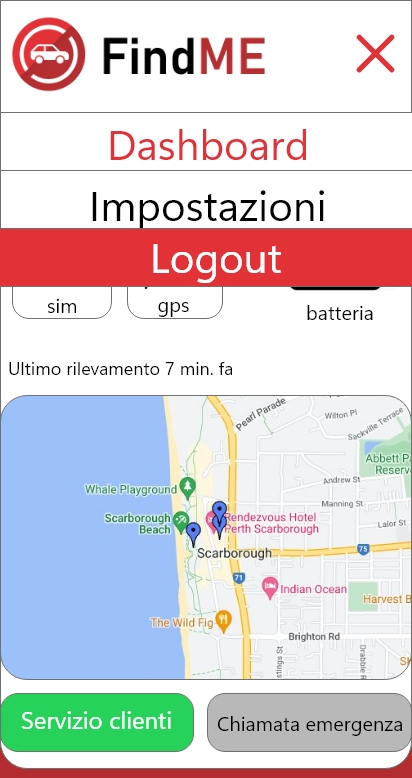
\includegraphics[width=0.9\linewidth]{img/dashboard-menu.jpg}}
  \caption{Dashboard home with menu opened}
  \label{fig:sub2}
\end{subfigure}
\caption{Dashboard view}
\label{fig:test}
\end{figure}


\subsection{Design architetturale}
Il sistema è composto da un servizio di backend che gestisce i dati e la business logic e un interfaccia di frontend per l'interazione con l'utente.\\


\section{Tecnologie}
Il sistema è stato realizzato utilizzando lo stack \textbf{MERN}.\\
Il backend è quindi basato su \textbf{Node.js} con l'impiego di \textbf{Express.js} per gestire le richieste e comunicare con il database non relazionale \textbf{MongoDB}. L'interfaccia utente è stata sviluppata con \textbf{React}.\\
La scelta di questa libreria è stata dettata dal fatto che nello studiare le tecnologie per il frontend proposti a lezione ho trovato più semplice apprendere il funzionamento di React.

\subsection{Backend}
Progettato per esporre un \textbf{API RESTful}.
\subsubsection{Persistenza}
Ottenuta tramite il database non relazionale MongoDB con il quale ci interfacciamo utilizzando la libreria \textbf{Mongoose}.\\
I dati immagazzinati sul database sono:
\begin{itemize}
    \item ultimo stato noto dei dispositivi;
    \item storico degli stati dei dispositivi durante i presunti furti;
    \item dati personali utente;
    \item dati veicolo (tra cui il codice univoco del dispositivo a cui sono associati).
\end{itemize}

\subsubsection{Autenticazione}
Gestita tramite \textbf{JSON Web Token}.\\
In risposta a login o registrazione con esito positivo viene mandato al client un \textbf{JWT}. Successivamente il client dovrà mandare questo token per ogni richiesta che necessita di autenticare l'utente richiedente. Il token viene immagazzinato all'interno del browser e può essere usato fino alla scadenza di questo o finchè il server non dovesse cambiare \textit{secret key}, quest'ultima viene generata casualmente all'avvio del server.

\subsubsection{Comunicazione event-based}
Vista la necessità di comunicare con gli utenti e con i dispositivi hardware in maniera event-based è stato deciso di usare la libreria \textbf{socket.io} presentata a lezione. Questa permette di comunicare tramite web socket. Nello specifico quando un dispositivo manda al server un aggiornamento riguardante il suo stato, questo viene salvato sulla memoria persistente (MongoDB) e successivamente inoltrato agli utenti associati a quel dispositivo che sono in ascolto.

\subsubsection{Notifiche in caso di furto}
Gestite tramite una API terza che permette di mandare email. Questa viene invocata tramite \textbf{Axios} inoltrando, come body, un html creato a partire da un template \textbf{PUG} contenente i dati dell'utente da notificare.

\subsection{Frontend}
Ho utilizzato diverse librerie e tecnologie:
\begin{itemize}
    \item \textbf{SCSS}: ha facilitato molto la scrittura e il mantenimento dei fogli di stile, ho usato i mixins per creare in modo facile dei temi (chiaro e scuro);
    \item \textbf{axios}: per comunicare agevolmente con il backend tramite l'interfaccia REST;
    \item \textbf{socket.io-client}: per ricevere aggiornamenti sullo stato del dispositivo comunicando con il backend tramite web-socket;
    \item \textbf{react-router}: per gestire il routing all'interno dell'applicazione;
    \item \textbf{framer motion}: per gestire animazioni e transizioni tra schermate diverse;
    \item \textbf{react-google-maps/api}: per visualizzare la posizione del dispositivo su una mappa;
\end{itemize}
insieme ad altri componenti e librerie che hanno avuto un ruolo meno rilevante.
\subsection{Dispositivo}
Il dispositivo è stato simulato per mezzo di un applicazione scritta per \textbf{Java 17.0.2}.\\
Questa consente di modificare tutti i parametri che utilizzerebbe il vero dispositivo per comunicare:
\begin{itemize}
    \item stato di batteria, segnale GPS e internet;
    \item presenza del beacon nelle vicinanze;
    \item se il veicolo è in movimento;
    \item l'indirizzo a cui mandare la richiesta tramite socket.io;
    \item il codice identificativo del dispositivo.
\end{itemize}
L'invio dello stato è gestito da un timer (la cui durata è modificabile). La posizione GPS che viene mandata è stata inserita arbitrariamente. Quando il dispositivo non è in allerta manda una posizione GPS fissa, quando è allertato manda ogni volta una posizione diversa seguendo l'ordine di una List riempita a mano in modo da simulare un percorso chiuso.

\section{Codice}
\subsubsection{Riusabilità component:}
Nel front-end il componente \textit{'MainHeader'} è stato volutamente creato in modo tale da permetterne una grande riusabilità, questo infatti è presente in tutte le schermate eccetto quelle di login/signup. Il suo compito è quello di di visualizzare il menu e di gestire le transizioni tra le diverse schermate all'interno della stessa react-route.\\
\subsubsection{Coerenza dati MongoDB:}
Visto che la coerenza dei dati è fondamentale in questa applicazione è stata utilizzata la funzionalità \textit{'Transaction}' offerta da MongoDB. Questa permette di fare commit delle modifiche durante la procedura di signin solo quando tutte le operazioni d'inserimento hanno avuto esito positivo, in caso contrario viene eseguito in automatico un rollback che invalida i nuovi dati e li rimuove dalle collezioni.\\
\subsubsection{Sicurezza stati Socket.io:}
Lo stato dei dispositivi (contenente anche le coordinate GPS) è un informazione sensibile e da proteggere. Questi dati vengono trasmessi mediante l'uso di \textit{Socket.io}, il client:
\begin{itemize}
    \item inizialmente richiede l'ultimo stato noto del dispositivo;
    \item successivamente si mette in attesa che il dispositivo mandi nuovi dati al server.
\end{itemize}
Nel primo caso il client viene autenticato per mezzo del JWT. Se l'autenticazione va a buon fine il socket viene inserito in una \textit{room} contenente i socket associati a username ed email dell'utente (dati che identificano univocamente un account).\\
Quando il server riceve aggiornamenti dal dispositivo, dopo averli salvati sul database, li inoltra a tutte le socket presenti nella room del proprietario del dispositivo previo controllo della validità dei token. Se il token di una o più socket della room scade, questa socket viene espulsa dalla room e la connessione viene interrotta.\\
\subsubsection{Sincronizzazione temporale tra backend e dispositivi client:}
Visto che il backend ed i client non sono sincronizzati temporalmente, nel component  \texttt{'DeviceInfo'} durante la callback eseguita alla recezione di dati dal server,  viene mascherata questa differenza per far sì che non sia visibile all'utente tramite la label indicante quando è stato ricevuto l'ultimo aggiornamento. La label non è comunque precisa visto che la sincronizzazione fatta non tiene conto del delay di trasmissione ma è comunque stato considerato abbastanza preciso ai fini della funzionalità in analisi. Una sincronizzazione vera e propria (es: tramite Lamport logical clock) è stata considerata non necessaria.


\section{Test}
Le funzionalità del sistema sono state testate su browser \textbf{Edge}, \textbf{Chrome} e \textbf{Firefox}.\\
L'accessibilità è stata verificata tramite \textbf{AChecker} e \textbf{W3C Validation Service}.\\
Le API RESTful sono state testate tramite l'uso di \textbf{Postman}.

\subsection{Euristiche di Nielsen}
L'usabilità dell'interfaccia è stata testata tramite la somministrazione di un questionario a 5 utenti reali.\\
Sono emerse le seguenti considerazioni:
\begin{itemize}
    \item \textbf{Visibilità dello stato del sistema}: il sistema informa sempre l'utente di cosa sta accadendo;
    \item \textbf{Corrispondenza tra sistema e mondo reale}: il linguaggio dell'applicazione è semplice e adatta a tutti;
    \item  \textbf{Controllo e libertà per l’utente}: le operazioni necessarie per portare a termine un task sono semplici da dedurre e il numero di operazioni è ridotto all essenziale;
    \item \textbf{Consistenza e standard}: consistenza nello stile visuale del sistema;
    \item \textbf{Prevenzione dall’errore}: l'utente non ha modo di incorrere in errori navigando l'interfaccia;
    \item \textbf{Riconoscimento più che ricordo}: i layout sono semplici, l'utente non deve adattarsi per fruire dell applicazione;
    \item  \textbf{Flessibilità ed efficienza}: la fruizione dell' applicazione è molto semplice, non servono scorciatoie;
    \item \textbf{Estetica e progettazione minimalista}: design minimale e chiaro;
    \item \textbf{Facilità di riconoscimento, diagnosi e risoluzione dalle situazioni di errore}: qualora ci fossero errori o mal funzionamenti questi vengono notificati e spiegati all utente. Insieme alla notifica c'è anche un suggerimento per risolvere il problema;
\end{itemize}
\subsection{Usability Test}
La correttezza dell'utilizzo del sistema è stata testata dallo sviluppatore e dagli utenti coinvolti nella fase di testing precedentemente descritta.
\subsection{Usability Test}
La bontà dell'esperienza utente è stata valutata tramite la somministrazione di un \textbf{UEQ} reperito su \href{https://www.ueq-online.org}{ueq-online.org} ai cinque utenti reali coinvolti. I risultati sono i seguenti:
\begin{figure}[H]
    \centering
    \frame{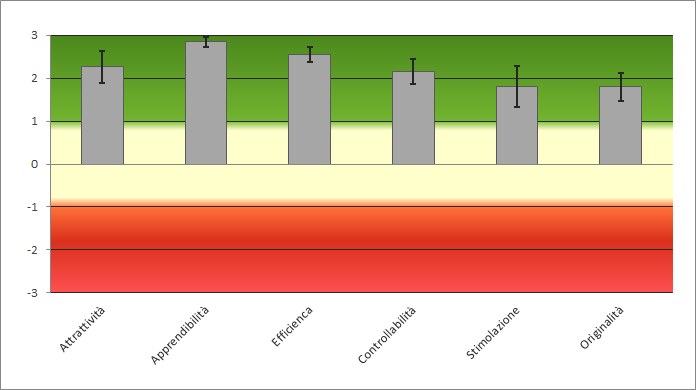
\includegraphics[width=1\linewidth]{img/grafico_UEQ.png}}\\
    \vspace{.5cm}
    \frame{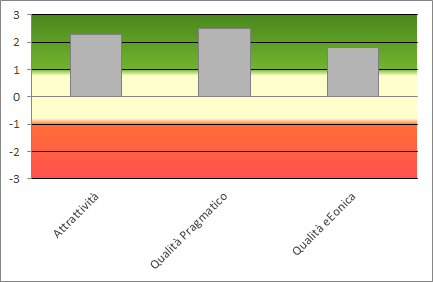
\includegraphics[width=1\linewidth]{img/grafico_UEQ_1.png}}
  \caption{risultati UEQ}
\end{figure}


\newpage
\section{Deployment}
L'applicazione è distribuita tramite l'utilizzo di \textbf{Docker}. Sono stati realizzati due container:
\begin{itemize}
    \item \texttt{node}: backend NodeJs contenente anche la build del frontend da inviare a fronte di determinate richieste;
    \item \texttt{mongo}: database MongoDB. La collection \texttt{car\_logos} che viene caricata in automatico al primo avvio del DB.
\end{itemize}
Tutto il materiale utilizzato per la creazione dei container è presente nel branch \texttt{main} di \href{https://bitbucket.org/davprs/anti-theft-system-for-vehicle/src/main/}{questa directory} Bitbucket.

\subsubsection{Setup}
Eseguire il comando:\\
\texttt{git clone -b deploy https://davprs@bitbucket.org/davprs/anti-theft-system-for-vehicle.git}\\
\newline
La struttura della directory è la seguente:\\
\dirtree{%
.1 anti-theft-system-for-vehicle.
.2 device-simulator.
.3 \framebox{Hardware\_Simulator.main.jar}.
.2 webApp.
.3 server.
.4 init-mongodb.
.5 data.
.6 car\_logos.json.
.5 init.sh.
.4 ASW\_saved.tgz.
.3 \framebox{docker\_load\_and\_run.bat}.
.3 \framebox{docker\_load\_and\_run.sh}.
.3 docker-compose.yml.
}
\hfill \break
I file evidenziati sono necessari per il setup e la fruizione del servizio.\\\break
In \texttt{device-simulator} è presente il simulatore di dispositivo in formato \textit{jar}.\\
In \texttt{webApp} va eseguito lo script \texttt{docker\_load\_and\_run.bat} (con Windows PowerShell) o \texttt{docker\_load\_and\_run.sh} a seconda del sistema operativo (rispettivamente Windows o Linux/MacOS). Questi script:
\begin{itemize}
    \item decomprimono l'archivio \texttt{ASW\_saved.tgz} contenente i salvataggi dei due container in formato \texttt{.tar};
    \item salvano i container come immagini Docker;
    \item eseguono i container.
\end{itemize}
Al termine dell esecuzione degli script basta aprire il browser e andare su \texttt{http://localhost:5000} per visualizzare la pagina web.\\
I container espongono le seguenti porte:
\begin{itemize}
    \item \textbf{5000}: richieste gestite da NodeJs ed Express;
    \item \textbf{4000}: richieste gestite da Socket.io;
    \item \textbf{27017}: MongoDB.
\end{itemize}

\section{Conclusioni}
Il sistema è semplice da utilizzare e svolge tutti i compiti richiesti e specificati dalle personas.\\ Per mancanza di tempo alcune funzionalità aggiuntive sono state eliminate in quanto non essenziali.\\Questo progetto si presta a molteplici estensioni e migliorie, quali ad esempio:
\begin{itemize}
    \item supporto all'utilizzo di multipli dispositivi per account;
    \item aggiunta di ruoli diversi da quello di \texttt{user} (es: amministratore di una flotta di veicoli);
    \item visualizzatore storico furti con i relativi percorsi.
\end{itemize}
\subsubsection{Commenti}
Questo progetto mi ha permesso di approfondire la conoscenza delle tecnologie e metodologie per lo sviluppo di applicazioni web moderne. Nello specifico mi è stato possibile migliorare le mie capacità e conoscenze riguardanti Docker, SCSS, React e JavaScript in generale.

\bibliographystyle{plain}
\bibliography{references}
\end{document}
